
\chapter{Fundamentação Teórica}

\section{Ensino Aprendizagem de Algoritmos em Portugol}

Portugol é uma pseudo linguagem algorítmica muito utilizada na descrição de
algoritmos, destaca-se por usar comandos em português, facilitando o aprendizado
da lógica de programação, e desta forma habituando o iniciante com o formalismo
da programação \cite{118}.

% FIX ME REESCREVER com minhas palavras "PLÁGIO" de {miranda2004}
Segundo \citeonline{manzanooliveira2005}, o portugol pode ser classificado como
uma técnica narrativa denominada de pseudocódigo, ou conhecida também por
português estruturado. Baseia-se em uma PDL - \textit{Program Design Language}
(Linguagem de Projeto de Programação), sendo que sua forma original de escrita é
conhecida como inglês estruturado, muito parecida com a notação da linguagem
PASCAL.

% FIX ME REESCREVER com minhas palavras "PLÁGIO" de {miranda2004}
Ainda segundo \citeonline{manzanooliveira2005}, o portugol é usado como
referência genérica para uma linguagem de projeto de programação, e tem por
finalidade mostrar uma notação para elaboração de algoritmos, que será usada na
definição, criação e desenvolvimento de uma linguagem computacional e sua
documentação.

% FIX ME REESCREVER com minhas palavras "PLÁGIO" de {miranda2004}
A representação de algoritmos em portugol, conforme \citeonline{118}, é rica em
detalhes, como a definição dos tipos das variáveis usadas no algoritmo,
encontrando muita aceitação por se assemelhar em demasia à forma em que são
escritos os programas.

% FIX ME REESCREVER com minhas palavras "PLÁGIO" de {miranda2004}
Comparando este processo aos fluxogramas destaca-se uma vantagem, visto que
segundo \citeonline{manzanooliveira2005}, é mais fácil escrever que desenhar
(na grande maioria dos casos), e a codificação acaba se tornando uma simples
transcrição de palavras chave. Corroborando \citeonline{118} aponta o fato do
Portugol ser uma linguagem simples e permitir o detalhamento dos algoritmos.
A tradução de um algoritmo em Portugol para um programa computacional através
de uma linguagem de programação fácil e clara, o que facilita muito o
ensino/aprendizagem da própria linguagem de programação. Outro destaque, é o
fato de a passagem para qualquer linguagem de programação ser quase imediata,
bastando ao aluno saber as palavras reservadas da respectiva linguagem de
programação.

% FIX ME REESCREVER com minhas palavras "PLÁGIO" de {miranda2004}
\citeonline{118} salienta que o inconveniente dos algoritmos é o fato de não
poderem ser executados no computador, pois o iniciante precisa imaginar a sua
execução, e essa tarefa não é fácil. \citeonline{souzaetal2000} apresenta outros
problemas, tais como a influência da linguagem de programação utilizada no
momento da definição do algoritmo e o fato de não haver utilização de recursos
visuais, o que deixa de estimular um fator importante no aprendizado dos alunos,
que é a visão.

\subsection{O Ensino de Algoritmos}

% FIX ME REESCREVER com minhas palavras "PLÁGIO" de {miranda2004}
O ensino de Algoritmos, em cursos de Computação, tem por objetivo ordenar o
pensamento do aluno, fazendo com que o mesmo aprenda a pensar na mesma sequência
lógica utilizada pelo computador. A importância dessa disciplina será percebida
mais tarde, quando o aluno iniciar o aprendizado em linguagens de programação e
precisar ordenar os passos para resolução de um problema, repassando-os ao
computador, sob forma de comandos \cite{miranda2004}.

% FIX ME REESCREVER com minhas palavras "PLÁGIO" de {miranda2004}
Conforme \citeonline{brookshear2000}, o algoritmo é uma codificação do
raciocínio necessário para resolver determinado problema, e essa capacidade
torna possível a construção de máquinas com comportamento inteligente – sendo
essa inteligência moldada através de software, o que torna a disciplina de
algoritmos essencial ao campo de Computação. O próximo passo seria representar
o algoritmo desenvolvido de uma forma apropriada ao entendimento da máquina ou
do aluno, através de comandos compreensíveis e sem ambiguidade, ou seja,
transportá-lo a uma linguagem de programação.

% FIX ME REESCREVER com minhas palavras "PLÁGIO" de {miranda2004}
\citeonline{003} coloca que o objetivo da disciplina de algoritmos é o aluno
desenvolver habilidades cognitivas que permitam que o mesmo aprenda a resolver
problemas, utilizando-se do computador como ferramenta. Os professores, seguindo
o raciocínio de \citeonline{003}, devem se preocupar com fatores como as
diferentes formas de resolução de um mesmo problema, e os diferentes estilos
cognitivos de um aluno. De acordo com \apudonline{gardner1984}{domingues2003},
cada ser humano possui um conjunto inato de competências intelectuais humanas
chamadas de Inteligências Múltiplas. Dentre estas inteligências, existe a
classificada como Lógico Matemática, chamada também de raciocínio científico ou
indutivo, que é a inteligência mais desenvolvida ou potencialmente mais
desenvolvida nos alunos dos cursos de Computação. \citeonline{003} ainda destaca
que o tipo de inteligência predominante em um indivíduo não irá padronizar seu
raciocínio ou a forma que o mesmo resolve problemas.

% FIX ME REESCREVER com minhas palavras "PLÁGIO" de {miranda2004}
O professor da disciplina de algoritmos, de acordo com \citeonline{003}, deve
conduzir a disciplina de forma que o próprio aluno descubra seu estilo de
raciocínio e forma de solução de problemas, auxiliando o aluno a modelar sua
solução em forma de algoritmo. Conforme \citeonline{menezesnobre2002}, o
professor da disciplina de algoritmos vivencia algumas dificuldades durante o
processo de aprendizagem, destacando-se:

% FIX ME REESCREVER com minhas palavras "PLÁGIO" de {miranda2004}
\begin{itemize}
  \setlength\itemsep{0em}
  \item reconhecer as habilidades inatas de seus alunos no processo de ensino;
  \item apresentar diferenciadas técnicas para solução dos problemas;
  \item trabalhar a capacidade do aluno de buscar soluções e escolha da
estrutura a ser utilizada; e
  \item promover a cooperação e colaboração entre os alunos.
\end{itemize}

% FIX ME REESCREVER com minhas palavras "PLÁGIO" de {miranda2004}
Outro problema seria a dificuldade dos alunos em abstrair do problema o que se
deseja. Normalmente, na disciplina de algoritmos, é dada a teoria, logo após
exemplos e exercícios referentes ao tema abordado. Estes exercícios normalmente
são constituídos de uma parte textual, situando o aluno no problema. A grande
dificuldade encontrada é abstrair deste texto o que se deseja, mais
especificamente, as entradas, o processamento e a saída \cite{miranda2004}.

% FIX ME REESCREVER com minhas palavras "PLÁGIO" de {miranda2004}
\citeonline{castrovcastrojr2002} salienta que a abordagem tradicional, que é o
curso baseado na programação imperativa, tem trazido sérios problemas aos alunos
que nunca programaram. Esta abordagem faz com que o aluno comece a pensar um
problema passo a passo, e isto não é o que é feito no dia a dia.
\citeonline{koliveretal2004} coloca que o despreparo da maior parte dos
estudantes em questão de enfrentar uma disciplina que pretende auxiliá-los no
desenvolvimento de soluções para problemas genéricos, em passos e de maneira
lógica, é um dos fatores para os altos índices de desistência e reprovação.

% FIX ME REESCREVER com minhas palavras "PLÁGIO" de {miranda2004}
\citeonline{koliveretal2004} informa que outro fator que causa dificuldade aos
professores é a heterogeneidade do público. Alguns acadêmicos possuem uma
engenhosidade superior nata, o que faz com que possuam uma facilidade natural
para a elaboração de soluções algorítmicas para problemas. Isso faz com que os
instrutores tenham problemas em questão de definição do programa da disciplina
e grau de complexidade dos problemas propostos.

% FIX ME REESCREVER com minhas palavras "PLÁGIO" de {miranda2004}
Dando sequência aos problemas encontrados, normalmente os professores utilizam
no ensino de algoritmos a pseudolinguagem Portugol, complementada pelo
fluxograma (até parte da disciplina). Parte dos alunos sentem dificuldades em
compreender estas estruturas. Conseguem analisar o problema, retirar dele as
entradas, processamento e saídas solicitadas, mas no momento de transportar para
a pseudolinguagem, sentem dificuldade em compreender de que forma isso deve ser
feito \cite{miranda2004}.

% FIX ME REESCREVER com minhas palavras "PLÁGIO" de {miranda2004}
Outro ponto interessante para ser analisado é a forma como os estudantes chegam
ao terceiro grau, conforme informa \citeonline{koliveretal2004}. Os calouros
normalmente chegam carregando vícios oriundos de práticas mecanicistas
frequentes nos primeiro e segundo graus, que acostuma o estudante a realizar
aplicações de fórmulas matemáticas sem realizar qualquer tipo de análise do
problema. Desta forma, o acadêmico entra na universidade sem conhecer um método
geral de resolução de problemas. Isto faz com que muitos professores da
disciplina possuam uma expectativa equivocada relativa ao conhecimento do aluno,
esperando que o mesmo possua habilidades para análise e resolução de problemas.
A ausência de disciplinas no ensino secundário que abordem a lógica também é um
fator determinante para os problemas encontrados. Mesmo aplicando a lógica no
dia a dia, grande parte dos estudantes possuem problemas ao aplicá-la de forma
satisfatória na construção de soluções algorítmicas sem os princípios básicos
que a norteiam.

% FIX ME REESCREVER com minhas palavras "PLÁGIO" de {miranda2004}
Por ser uma disciplina inicial, e uma disciplina com um grau de dificuldade
grande para os alunos que não conseguem se adaptar à forma de pensamento passo
a passo, muitas vezes o professor sente dificuldades, durante as aulas, de
avaliar qual é o problema encontrado pelos alunos. Normalmente as turmas de
algoritmos são turmas grandes, e a maior parte dos alunos não evidenciam de
forma verbal os problemas encontrados. Essas dúvidas somente se tornam claras
durante a aplicação de uma prova ou mesmo de exercícios válidos como nota
\cite{miranda2004}.

% FIX ME REESCREVER com minhas palavras "PLÁGIO" de {miranda2004}
Pode-se também citar, como problema, a questão da correção de provas e
exercícios que o professor aplica aos alunos. Como citado anteriormente,
normalmente as turmas da disciplina de Algoritmos são turmas grandes, primeiro
por ser uma disciplina ministrada no primeiro período - portanto, todos os
alunos que ingressam através do vestibular matriculam-se nela -, pelo alto
índice de reprovação. Ao corrigir provas de algoritmos, o professor deve levar
em consideração que cada aluno resolve problemas de formas diferentes,
portanto, um mesmo problema pode possuir diversos caminhos de resolução, e
avaliar todos os problemas um a um, estabelecendo um padrão para a correção.
Mas devido a grande quantidade de provas a serem corrigidas o professor,
involuntariamente, poderá alterar a forma de avaliação de um aluno para outro
\cite{miranda2004}.

% FIX ME REESCREVER com minhas palavras "PLÁGIO" de {miranda2004}
Apesar dos problemas citados anteriormente, a disciplina de algoritmos, baseada
em Portugol e fluxograma, ainda é ministrada na grande maioria dos cursos de
Computação, pois através dela o aluno consegue ter embasamento para aprender
diversas linguagens de programação. A disciplina de algoritmos em si ensina o
aluno a compreender um problema, definir sua resolução e aplicar esta resolução
no formato da pseudo linguagem. Na grande maioria das vezes, juntamente ao
ensino de Algoritmos é ensinado aos acadêmicos alguma linguagem de programação,
normalmente C ou Pascal. Com o algoritmo elaborado, torna-se mais fácil o
desenvolvimento do programa, pois a parte essencial, a parte lógica do problema,
já está resolvida. Portanto, o aluno deve somente transferir a resolução para a
linguagem de programação \cite{miranda2004}.

\section{O Ensino da Linguagem de Programação Portugol}

O ensino da lógica de programação geralmente é tratado nas primeiras fases dos
cursos de informática, onde os alunos iniciantes aprendem a desenvolver o
raciocínio lógico para então escrever algoritmos para solução de problemas. O
Portugol é uma pseudo linguagem algorítmica muito utilizada na descrição de
algoritmos, destaca-se pelo uso de comandos em português, o que facilita o
aprendizado da lógica de programação, habituando o iniciante com o formalismo de
programação.

% FIX ME REESCREVER com minhas palavras "PLÁGIO" de {118}
Apesar de todas essas vantagens, o Portugol apresenta o inconveniente dos
algoritmos não poderem ser executados no computador. Dessa forma, o iniciante
precisa imaginar a sua execução, o que não é uma tarefa tão fácil para quem está
começando.

% FIX ME REESCREVER com minhas palavras "PLÁGIO" de {118}
A lógica para programação consiste em aprender a pensar na mesma sequência em
que o computador executa as tarefas, aprende-se a imaginar como as ações serão
executadas partindo-se do estudo de um problema até chegar a construção de um
algoritmo (solução). Considere com exemplo o seguinte problema:

% FIX ME REESCREVER com minhas palavras "PLÁGIO" de {118}
``Expressar o resultado da soma de dois valores.''

% FIX ME REESCREVER com minhas palavras "PLÁGIO" de {118}
É comum, para uma pessoa pensar em algo assim:

% FIX ME REESCREVER com minhas palavras "PLÁGIO" de {118}
``Pegar os dois valores, somar e dar o resultado.''

% FIX ME REESCREVER com minhas palavras "PLÁGIO" de {118}
Após ter adquirido uma certa experiência, a mesma pessoa pode, de forma
automática, converter tal pensamento em instruções sem necessidade de especificar
detalhadamente os processos que estão implícitos nesta pequena rotina (ver tabela \ref{tab:action+operation}):

% FIX ME REESCREVER com minhas palavras "PLÁGIO" de {118}
\begin{table} [!htb]
  \caption{Ações e Operações}\label{tab:action+operation}
  \centering
  %\begin{tabular}{| m{2.4cm} | m{10.9cm}|}\hline
  \begin{tabular}{ m{2.4cm} | m{10.9cm} }\hline
  %\rowcolor{black!20}\Centering\bfseries Ações & \Centering\bfseries Operações \\ \hline
  \bfseries Ações & \bfseries Operações \\ \hline
  \MakeTextUppercase{Pegar} & Receber os dois valores numéricos e armazená-los \\ \hline
  \MakeTextUppercase{Somar} & Executar a instrução de soma e armazenar o resultado \\ \hline
  \MakeUppercase{Dar o \mbox{Resultado}} & Mostrar o resultado, armazená-lo para o uso
  posterior ou para ser visualizado em outra oportunidade \\
  \hline
  \end{tabular}
  \caption*{\footnotesize Fonte: Farrer (1989)}
\end{table}

% FIX ME REESCREVER com minhas palavras "PLÁGIO" de {118}
Quanto maior o domínio da lógica de programação, mais fácil será detalhar as
tarefas envolvidas na solução do problema proposto e mais eficiente será o
algoritmo criado, porém, para um iniciante construir um algoritmo que permita
a um computador executar a tarefa proposta não é tão simples.

% FIX ME REESCREVER com minhas palavras "PLÁGIO" de {118}
Segundo \cite[p. 17]{farreretal1989}: ``Algoritmo é a descrição de um conjunto de comandos que, obedecidos, resultam numa sucessão finita de ações''.
A tabela \ref{tab:action+operation}, mostra duas leituras de um algoritmos, uma bastante genérica (ações) e outro um pouco mais detalhada (operações), porém, apesar de apresentar um bom nível de detalhamento ainda não pode ser considerado um algoritmo para o computador. Em Portugol, o mesmo algoritmo pode ser escrito da seguinte forma:

%\DeclareRobustCommand{\Attribuition}{\text{\reflectbox{$\ding{212}$}}}

%\reflectbox{$\ding{212}$}
%\text{\reflectbox{$\ding{212}$}}

% FIX ME REESCREVER com minhas palavras "PLÁGIO" de {118}
\begin{lstlisting}[]  % Start your code-block

Algoritmo exemplo;
Var v1 ,v2 , v3 : inteiro;
Inicio
  leia (v1);
  leia (v2);
  v3 <- v1 + v2;
  escreva (v3);
Fim.
\end{lstlisting}

% FIX ME REESCREVER com minhas palavras "PLÁGIO" de {118}
A representação dos algoritmos em Portugol, conhecido também como pseudocódigo,
é muito utilizada, segundo \cite[p.~6]{saliba1992}: ``Esta forma de
representação de algoritmo é rica em detalhes, como a definição dos tipos das
variáveis usadas no algoritmo e, por assemelhar-se bastante à forma em que os
programas são escritos, encontra muita aceitação.''

% FIX ME REESCREVER com minhas palavras "PLÁGIO" de {118}
A tradução de um algoritmo escrito em Portugol para um programa de computador
numa linguagem de programação é muito fácil e clara, facilitando assim o ensino
e aprendizado da linguagem de programação. O Portugol é a forma mais utilizada
para escrever algoritmos por ser uma linguagem simples e permitir o
detalhamento dos algoritmos.

% FIX ME REESCREVER com minhas palavras "PLÁGIO" de {118}
O ensino do Portugol, hoje, em muitos casos é feito de maneira manual
(utilizando folhas de papel), o que não estimula os alunos em aprender e
exercitar o desenvolvimento de algoritmos.

\subsection{A Ferramenta Portugol/Plus}

% FIX ME REESCREVER com minhas palavras "PLÁGIO" de {118}
O Objetivo principal do sistema Portugol/Plus é fornecer uma ferramenta de apoio
ao ensino da lógica de programação baseado no Portugol, sem reduzir o estudo
teórico. Com esta ferramenta pretende-se proporcionar uma forma de estimular os
alunos a praticar e exercitar o desenvolvimento de algoritmos em Portugol.

% FIX ME REESCREVER com minhas palavras "PLÁGIO" de {118}
O ambiente foi desenvolvido para operar em microcomputador do tipo PC
(\textit{Personal Computer}), sob o sistema operacional DOS
(\textit{Disk Operating System}), e divide-se em duas partes principais:

% FIX ME REESCREVER com minhas palavras "PLÁGIO" de {118}
\begin{itemize}
  \setlength\itemsep{0em}
  \item Editor de algoritmos (padrão ASCII);
  \item Compilador.
\end{itemize}

\begin{enumerate}
% FIX ME REESCREVER com minhas palavras "PLÁGIO" de {118}
  {\bfseries\item Editor de Algoritmos:}

% FIX ME REESCREVER com minhas palavras "PLÁGIO" de {118}
  \begin{figure}[h]
    \centering
    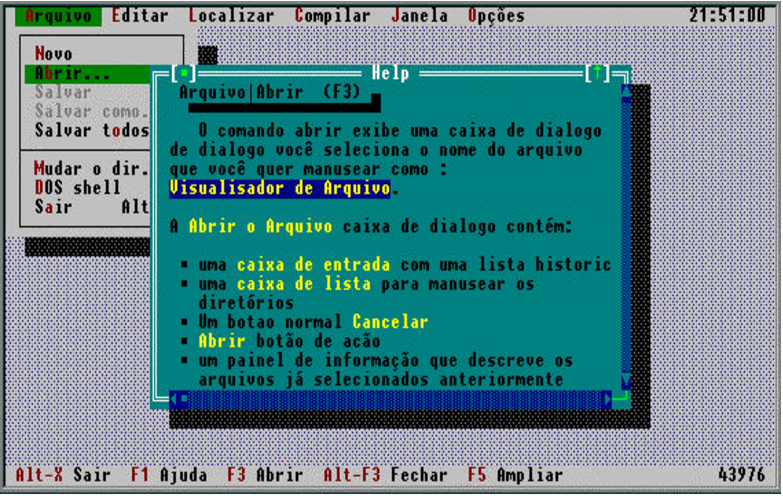
\includegraphics{figures/portugolplus-ambiente.pdf}
    \caption{Visão Geral do Ambiente}\label{fig:portugolplus-ambiente}
  \end{figure}

% FIX ME REESCREVER com minhas palavras "PLÁGIO" de {118}
O editor de algoritmos, permite a digitação e a manipulação dos arquivos que
contém os algoritmos utilizando uma interface dirigida por menus. Numa visão
geral (figura \ref{fig:portugolplus-ambiente}) vê-se os diversos menus (Arquivo,
Editar, Localizar, Compilar, Janela e Opções):

\begin{itemize}

% FIX ME REESCREVER com minhas palavras "PLÁGIO" de {118}
  \item O menu arquivos permite, como o nome diz, a manutenção de arquivos, com
  itens como criar, salvar e salvar como (salvar com outro nome), contando também
  com ações extras, tais como:

\begin{itemize}

% FIX ME REESCREVER com minhas palavras "PLÁGIO" de {118}
  \item Mudar o dir que serve para alterar o diretório (área de trabalho) em que
  o ambiente pesquisa os arquivos para edição.

% FIX ME REESCREVER com minhas palavras "PLÁGIO" de {118}
  \item Dos shell que serve para se obter uma sessão de linha de comando do
  sistema operacional sem abandonar o ambiente.

% FIX ME REESCREVER com minhas palavras "PLÁGIO" de {118}
  \item Sair para encerrar a execução do ambiente.

\end{itemize}

% FIX ME REESCREVER com minhas palavras "PLÁGIO" de {118}
  \item O menu editar permite executar ações sobre os arquivos em edição
  (abertos), estas ações compreendem copiar, mudar e/ou apagar partes dos
  arquivos em edição.

% FIX ME REESCREVER com minhas palavras "PLÁGIO" de {118}
  \item O menu localizar ajuda na busca e/ou substituição de trechos escritos no
  arquivo atual em uso (corrente).

% FIX ME REESCREVER com minhas palavras "PLÁGIO" de {118}
  \item O menu janela controla o modo como são visualizados todos os arquivos
  abertos (em edição) em um mesmo instante.

% FIX ME REESCREVER com minhas palavras "PLÁGIO" de {118}
  \item O menu opções controla valores configuráveis pelo usuário dentro do
  ambiente como cores e mouse.

% FIX ME REESCREVER com minhas palavras "PLÁGIO" de {118}
  \item O menu opções controla valores configuráveis pelo usuário dentro do
  ambiente como cores e mouse.

% FIX ME REESCREVER com minhas palavras "PLÁGIO" de {118}
  \begin{figure}[h]
    \centering
    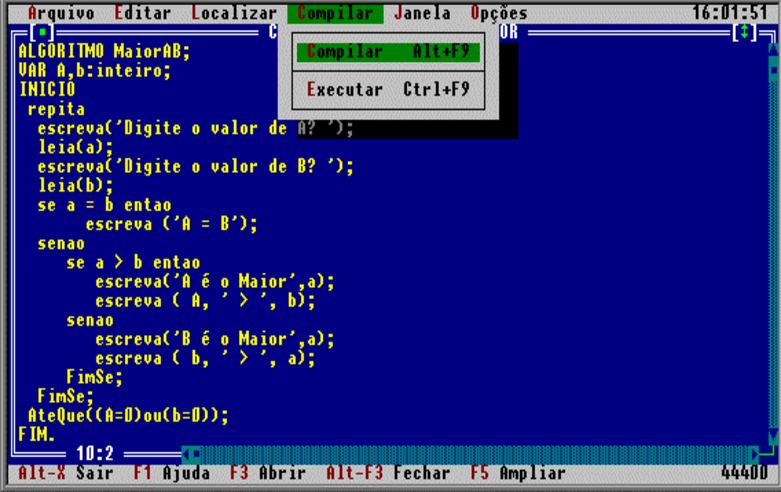
\includegraphics{figures/portugolplus-compilar.pdf}
    \caption{Visão do Menu Compilar}\label{fig:portugolplus-compilar}
  \end{figure}

% FIX ME REESCREVER com minhas palavras "PLÁGIO" de {118}
  \item O menu compilar (figura \ref{fig:portugolplus-compilar}), serve para
  tornar possível a execução dos algoritmos criados. Após editado e salvo,
  usa-se este menu para a realização da compilação do algoritmo, depois de
  corrigidos os erros (caso seja encontrado algum), pode-se executar o algoritmo
  para ver o seu comportamento, se o resultado obtido é realmente o desejado.
  Podendo-se também, o que é muito importante para o aprendizado, partir para
  sucessivos refinamentos (melhorias) nas soluções encontradas, sempre tendo-se
  a possibilidade de visualizar como as alterações feitas afetam o resultado
  pretendido (a nova solução pode vir a ser melhor, pior ou equivalente).

\end{itemize}

  {\bfseries\item Compilação:}

% FIX ME REESCREVER com minhas palavras "PLÁGIO" de {118}
O conhecimento sobre a construção de compiladores, segundo
\cite{ahoetal1995,joseneto1987}, remonta do início da década de 50, não se
sabendo precisamente o seu início. A construção de compiladores foi motivada
pela complexidade de programar em computadores na época, quando usava-se código
de máquina ou Assembler, o que  além de difícil, forçava a execução do programa
no equipamento para o qual o mesmo havia sido escrito, pois em outros o código
precisava ser reescrito, o que resultava em versões do mesmo programa para cada
tipo de equipamento.

% FIX ME REESCREVER com minhas palavras "PLÁGIO" de {118}
Os compiladores são programas que recebem com entrada um programa fonte,
analisam-no o conteúdo e o contexto, caso encontrem erros informam ao usuário,
do contrário, convertem o programa fonte para um programa objeto geralmente em
linguagem da máquina.

% FIX ME REESCREVER com minhas palavras "PLÁGIO" de {118}
O compilador trabalha sobre uma gramática, que é um conjunto de palavras
(instruções) limitado por ele e reconhecidas como comandos, que tem regras fixas
e não conflitantes de uso, o que significa que uma instrução tem apenas um
significado para um compilador, não havendo ambiguidade.

% FIX ME REESCREVER com minhas palavras "PLÁGIO" de {118}
  \begin{figure}[h]
    \centering
    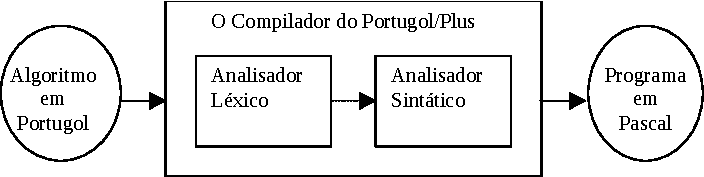
\includegraphics{figures/portugolplus-compilador.pdf}
    \caption{O Compilador}\label{fig:portugolplus-compilador}
  \end{figure}

% FIX ME REESCREVER com minhas palavras "PLÁGIO" de {118}
Durante o processo de compilação como mostrado na figura 3, o compilador do
ambiente Portugol/Plus faz uma verificação da sintaxe das instruções usadas no
algoritmo, caso não sejam encontrados erros, um programa objeto é gerado na
linguagem de programação Pascal \cite{farreretal1995}. Através de um compilador
Pascal executa-se o programa objeto.

\end{enumerate}

% FIX ME REESCREVER com minhas palavras "PLÁGIO" de {118}
A programação de computador, não é algo muito complexo de ser aprendida, no
entanto, para o seu aprendizado é necessário dominar a lógica de programação.
O ensino da lógica depara-se hoje com uma problemática, que é a falta de
experimentar na prática o que é estudado na teoria. A falta de prática
desestimula os alunos iniciantes a aprofundar no conteúdo a ser aprendido
\cite{118}.

% FIX ME REESCREVER com minhas palavras "PLÁGIO" de {118}
Visando a melhoria do ensino da lógica foi desenvolvido o Portugol/Plus, que
é um sistema que auxilia na tarefa de ensinar e estudar a lógica de programação.
Ele estimula o aluno a praticar e exercer o desenvolvimento de algoritmos,
facilitando assim o trabalho do professor e também ajudando o aluno a ter um
domínio melhor sobre o assunto \cite{118}.

% FIX ME REESCREVER com minhas palavras "PLÁGIO" de {118}
O principal público alvo são os alunos iniciantes dos cursos de Informática,
onde se espera, com a utilização desta ferramenta, um aumento no domínio do
conteúdo da lógica \cite{118}.

\section{Processamento de Linguagem Natural}

% FIX ME REESCREVER com minhas palavras "PLÁGIO" de {mirandaetal2005}
\citeonline{barrfeigengaum1986} colocam que o caminho mais comum para que as
pessoas se comuniquem é falando ou escrevendo através de linguagem natural, seja
em inglês, francês, português ou chinês. As linguagens de computadores possuem
um formato mais rígido, para que possam ser convertidas em uma seqüência de
instruções de computador. O estudo de processamento de linguagem natural procura
fazer com que os computadores possam entender a linguagem natural humana,
tornando-se mais fáceis de utilizar.
